\subsection{Kernels}
\label{subsection:kernels}
Kernels are just the weightings that define the characteristics of a filter, also known as a filter's mask. A filter kernel is nearly always square so as to have a center cell which sits atop a reference pixel. The result of the filter's application at that reference pixel will be stored in the output image at the location of the reference pixel. Notice in Figure \ref{fig:kernel_graphics} how the mask sits over the reference pixel.

% TREE %
\begin{figure}[H]
 \centering
 \centering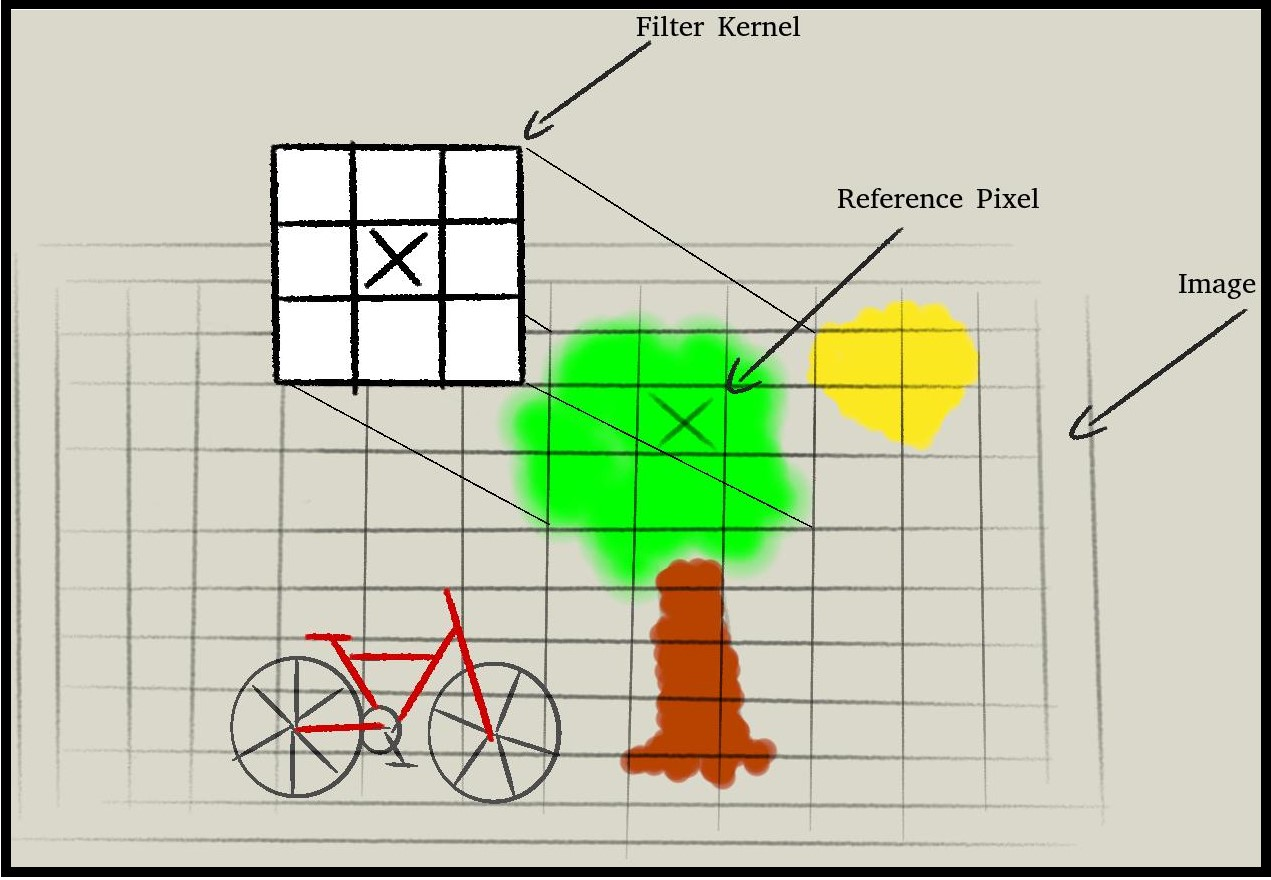
\includegraphics[width=350pt]{kernel_graphics}
 \caption{Visualization of a Filter Kernel Application}
 \label{fig:kernel_graphics}
\end{figure}

\subsubsection{Box Filter}
\label{subsubsection:boxfilter}
A box filter also known as a moving average filter simply outputs the average of its inputs because the filter weights are evenly distributed (Figure \ref{fig:box_kernel}). By passing this filter over an image its sharpness is reduced because the filter flattens out difference in values generating a smooth effect which can be observed in Figure \ref{fig:pug_blur}. This filter's 'flattening' effect is useful for removing noise which stands out from other pixel values.


% DOG BOX FILTERED%
\begin{figure}[H]
    \centering
    \begin{subfigure}[b]{0.3\textwidth}
        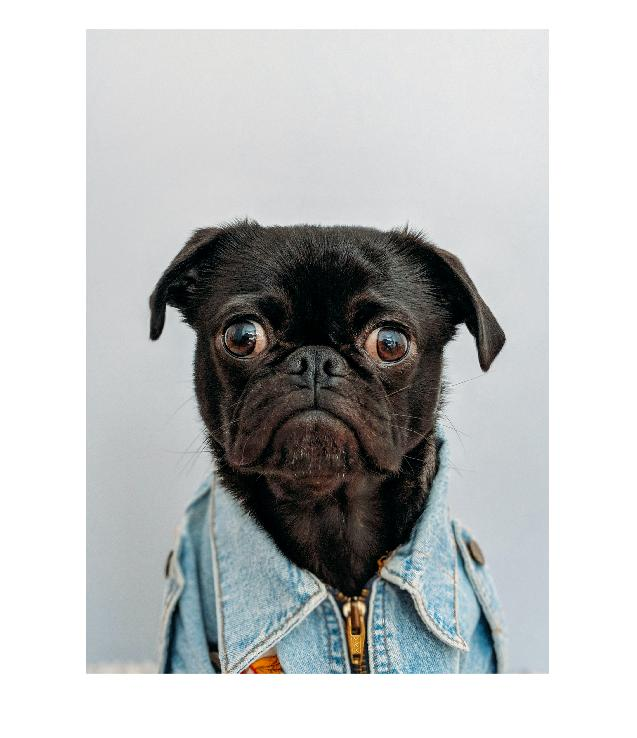
\includegraphics[width=\textwidth]{pug_resized}
        \caption{Img: Charles Deluvio}
        \label{fig:pug_noise}
    \end{subfigure}
    \begin{subfigure}[b]{0.3\textwidth}
        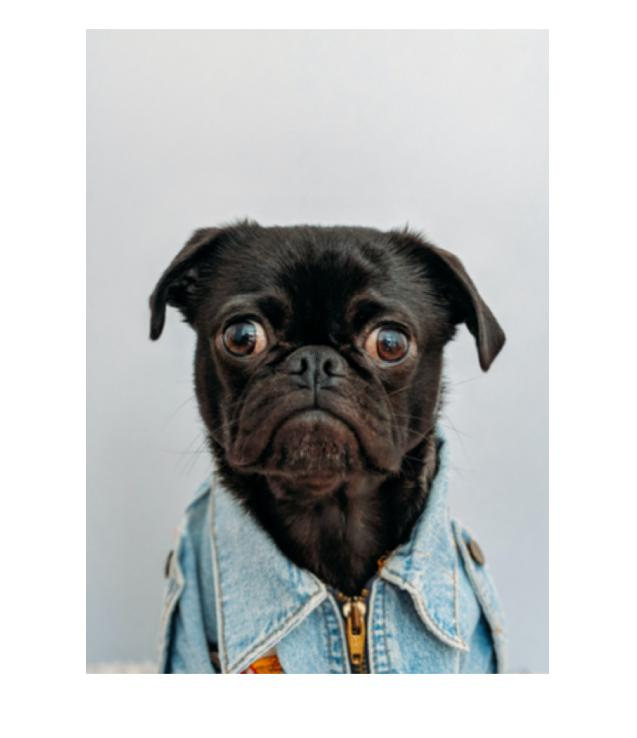
\includegraphics[width=\textwidth]{pug_blur}
        \caption{Blurred pug}
        \label{fig:pug_denoised}
    \end{subfigure}
    \caption{Application of a 17x17 Box filter to blur image.}
    \label{fig:pug_blur}
\end{figure}

\begin{figure}[H]
   \centering
   \[
     \frac{1}{9}
   \begin{bmatrix}
      1 & 1 & 1 \\
      1 & 1 & 1 \\
      1 & 1 & 1
   \end{bmatrix}
   \]
   \caption{3x3 Box Filter Kernel}
   \label{fig:box_kernel}
\end{figure}

\subsubsection{Gaussian Kernel}
\label{subsubsection:gauss_kernel}
The Gaussian is a significant kernel in image processing as it is good at filtering out noise. This kernel models the Gaussian function (see Section \ref{section:gaussian}) or normal distribution. It works in a similar fashion to the moving average filter but is superior at filtering noise as it addresses two properties about images that are generally true, 

\begin{enumerate}
    \item The 'real' value of a pixel is probably the same or similar to its neighbors. 
    \item Each pixel of noise in an image is added independently.
\end{enumerate}

The Gaussian addresses both of these qualities by having high value cooefficients at the filter's center and lower values tapering out to the edges of the filter (Figure \ref{fig:gauss_kernel}). This means that values closer together are more strongly correlated than those further away from the reference pixel as can be observed in the 7x7 Gaussian filter kernel in Figure \ref{fig:pug_noise}.

% SOBEL FILTER APPLICATION
\begin{figure}[H]
    \centering
    \begin{subfigure}[b]{0.3\textwidth}
        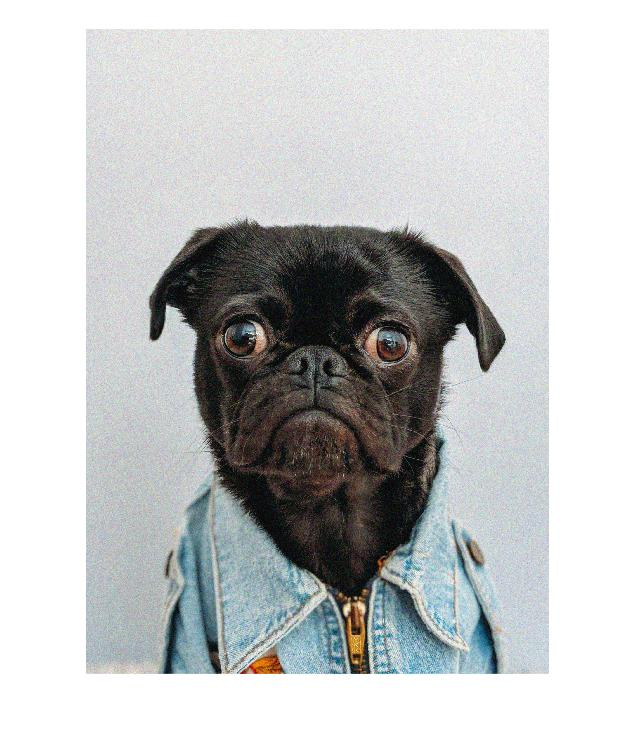
\includegraphics[width=\textwidth]{pug_noise}
        \caption{Noisey pug}
        \label{fig:pug_noise}
    \end{subfigure}
    \begin{subfigure}[b]{0.3\textwidth}
        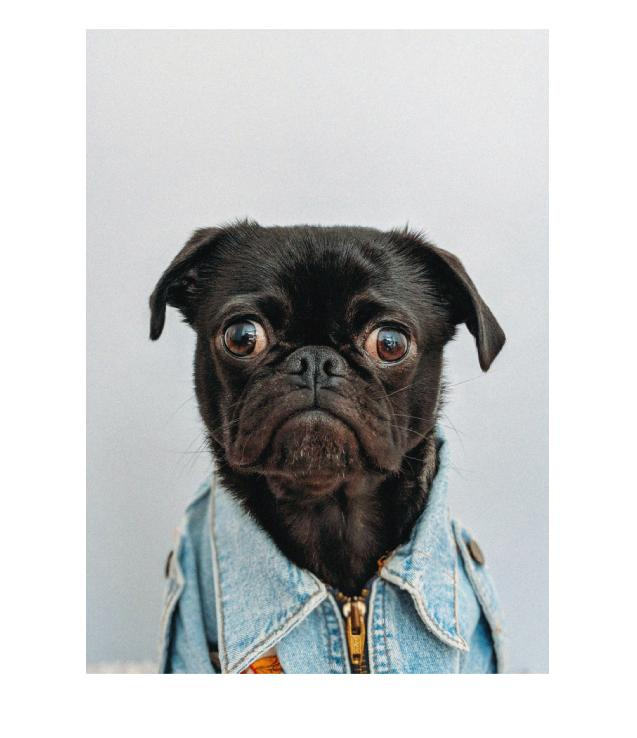
\includegraphics[width=\textwidth]{pug_denoised}
        \caption{Denoised pug}
        \label{fig:pug_denoised}
    \end{subfigure}
    \caption{Application of a 7x7 Gaussian filter to denoise image.}
    \label{fig:pug_noise}
\end{figure}


\begin{figure}[H]
    \centering
    \[
    \begin{bmatrix}
       0 & 0 & 0 & 0 & 0 & 0 & 0 \\
       0 & 0 & 0 & 0.0002 & 0 & 0 & 0 \\
       0 & 0 & 0.0113  & 0.0837 & 0.0113  & 0 & 0 \\
       0 & 0.0002 & 0.0837 & 0.6187 & 0.0837 & 0.0002 & 0 \\
       0 & 0 & 0.0113 & 0.0837 & 0.0113 & 0 & 0 \\
       0 & 0 & 0 & 0.0002 & 0 & 0 & 0 \\
       0 & 0 & 0 & 0 & 0 & 0 & 0 \\
    \end{bmatrix}
    \]
    \caption{7x7 Gaussian Filter Kernel, Sigma = 0.5}
    \label{fig:gauss_kernel}
\end{figure}